\chapter{Python's Object Oriented Programming}\label{introduction-to-python---lesson-2}

In this chapter the main characteristics that makes $\tt{python}$ an \textit{object oriented programming} language will be reviewed.
Before going to OOP however the concepts of function and variable scope will be outlined.

\section{Functions}\label{functions}

A function is a block of organized, reusable code that is used to perform a single action. Functions provide better modularity for your application and high degree of code reusing.
To define a function the keyword \texttt{def} is used, followed by the name of the function and by the required parameters in parenthesis. Functions are called by name passing the necessary parameters if any.

\begin{tcolorbox}[breakable, size=fbox, boxrule=1pt, pad at break*=1mm,colback=cellbackground, colframe=cellborder]
\begin{Verbatim}[commandchars=\\\{\}]
\PY{c+c1}{\PYZsh{} sum up all the integers between 1 and n }
\PY{k}{def} \PY{n+nf}{my\PYZus{}function}\PY{p}{(}\PY{n}{n}\PY{p}{)}\PY{p}{:} \PY{c+c1}{\PYZsh{} this function take one input only (n)}
    \PY{n}{x} \PY{o}{=} \PY{l+m+mi}{0}
    \PY{k}{for} \PY{n}{i} \PY{o+ow}{in} \PY{n+nb}{range}\PY{p}{(}\PY{l+m+mi}{1}\PY{p}{,} \PY{n}{n}\PY{o}{+}\PY{l+m+mi}{1}\PY{p}{)}\PY{p}{:}
        \PY{n}{x} \PY{o}{+}\PY{o}{=} \PY{n}{i}
    \PY{k}{return} \PY{n}{x} \PY{c+c1}{\PYZsh{} the function returns a number}

\PY{n}{my\PYZus{}function}\PY{p}{(}\PY{l+m+mi}{5}\PY{p}{)} \PY{c+c1}{\PYZsh{} 5 + 4 + 3 + 2 + 1}
\end{Verbatim}
\end{tcolorbox}

Functions can return any kind of objects (numbers, strings, lists, complex objects\ldots{}) but it is not mandatory to have a return value, so you can have functions \textbf{without} a \texttt{return} statement (e.g. a function that simply take a string as input and print it to screen with a particular format).
In addition the syntax of the \texttt{return} is different from other languages like \texttt{Visual\ Basic}, the returned object doesn't have to have the same name as the function. Indeed above the variable $\tt{x}$ is returned and not the variable \texttt{my\_function}. Below an example of function not returning anything.

\begin{Shaded}
\begin{Highlighting}[]
\KeywordTok{def}\NormalTok{ printing(mystring):}
    \BuiltInTok{print}\NormalTok{((myString)}\BuiltInTok{.upper())}
\end{Highlighting}
\end{Shaded}

Functions can call other functions (once a function has been defined it can be accessed from everyone within the same file or notebook): here $\tt{my\_function_2}$ calls $\tt{my\_function}$

\begin{tcolorbox}[breakable, size=fbox, boxrule=1pt, pad at break*=1mm,colback=cellbackground, colframe=cellborder]
\begin{Verbatim}[commandchars=\\\{\}]
\PY{k}{def} \PY{n+nf}{my\PYZus{}function\PYZus{}2}\PY{p}{(}\PY{n}{n}\PY{p}{,} \PY{n}{x}\PY{p}{)}\PY{p}{:} 
   \PY{k}{return} \PY{l+s+s2}{\PYZdq{}}\PY{l+s+s2}{The result is : }\PY{l+s+si}{\PYZob{}\PYZcb{}}\PY{l+s+s2}{\PYZdq{}}\PY{o}{.}\PY{n}{format}\PY{p}{(}\PY{n+nb}{str}\PY{p}{(}\PY{n}{my\PYZus{}function}\PY{p}{(}\PY{n}{n}\PY{p}{)}\PY{o}{*}\PY{n}{x}\PY{p}{)}\PY{p}{)}

\PY{n}{my\PYZus{}function\PYZus{}2}\PY{p}{(}\PY{l+m+mi}{5}\PY{p}{,} \PY{l+m+mi}{10}\PY{p}{)}
\end{Verbatim}
\end{tcolorbox}

Functions can also call themselves too (i.e \emph{recursion}). In the next example we will see a function that computes the factorial exploiting the following relationship:

\[
\begin{cases}
    n! = n \times (n-1)! & \;\; (\forall n \gt 1) \\
    n! = 1 & \;\; (\forall n \le 1)
\end{cases}
\]

\begin{tcolorbox}[breakable, size=fbox, boxrule=1pt, pad at break*=1mm,colback=cellbackground, colframe=cellborder]
\begin{Verbatim}[commandchars=\\\{\}]
\PY{k}{def} \PY{n+nf}{factorial}\PY{p}{(}\PY{n}{n}\PY{p}{)}\PY{p}{:}
   \PY{k}{if} \PY{n}{n} \PY{o}{\PYZlt{}}\PY{o}{=} \PY{l+m+mi}{1}\PY{p}{:}
      \PY{k}{return} \PY{l+m+mi}{1}
   \PY{k}{else}\PY{p}{:}
      \PY{k}{return} \PY{n}{n} \PY{o}{*} \PY{n}{factorial}\PY{p}{(}\PY{n}{n}\PY{o}{\PYZhy{}}\PY{l+m+mi}{1}\PY{p}{)}

\PY{n}{factorial}\PY{p}{(}\PY{l+m+mi}{10}\PY{p}{)}
\end{Verbatim}
\end{tcolorbox}

In this example the function $\tt{factorial}$ is initially called with the input corresponding to the factorial we want to compute, it then call itself each time with $\tt{n-1}$, multiplying together all the results.
The previous example is quite simple but recursion can be tricky sometimes so apply it with caution. 

Functions input parameters can have default values, which means that a function that works with some input values can be called with less parameters provided their default values have been specified.

In the following example the function $\tt{powers}$ takes three inputs: a list of numbers, an exponent ($\tt{n}$) and a constant ($\tt{c}$). The code loops through the provided list of numbers and process them according to the formula $item^{n} + c$, it puts the results in a new list which will be finally returned.

\begin{tcolorbox}[breakable, size=fbox, boxrule=1pt, pad at break*=1mm,colback=cellbackground, colframe=cellborder]
\begin{Verbatim}[commandchars=\\\{\}]
\PY{k}{def} \PY{n+nf}{powers}\PY{p}{(}\PY{n}{l}\PY{p}{,} \PY{n}{n}\PY{o}{=}\PY{l+m+mi}{2}\PY{p}{,} \PY{n}{c}\PY{o}{=}\PY{l+m+mi}{0}\PY{p}{)}\PY{p}{:}
    \PY{k}{return} \PY{p}{[}\PY{n}{item}\PY{o}{*}\PY{o}{*}\PY{n}{n}\PY{o}{+}\PY{n}{c} \PY{k}{for} \PY{n}{item} \PY{o+ow}{in} \PY{n}{l}\PY{p}{]}

\PY{n+nb}{print} \PY{p}{(}\PY{n}{powers}\PY{p}{(}\PY{p}{[}\PY{l+m+mi}{5}\PY{p}{,} \PY{l+m+mi}{11}\PY{p}{,} \PY{l+m+mi}{6}\PY{p}{]}\PY{p}{,} \PY{l+m+mi}{3}\PY{p}{,} \PY{l+m+mi}{4}\PY{p}{)}\PY{p}{)}
\PY{n+nb}{print} \PY{p}{(}\PY{n}{powers}\PY{p}{(}\PY{p}{[}\PY{l+m+mi}{5}\PY{p}{,} \PY{l+m+mi}{11}\PY{p}{,} \PY{l+m+mi}{6}\PY{p}{]}\PY{p}{)}\PY{p}{)}

[129, 1335, 220]
[25, 121, 36]
\end{Verbatim}
\end{tcolorbox}
    
As you can see the function is called twice with two different set of parameters: in the first case we pass to it the list of numbers, the exponent and the constant, in the second just the same list of numbers.
In the latter case, being defined the default values for $\tt{n}$ and $\tt{c}$, the function works perfectly well, fewer inputs are provided and the missing ones are replaced by their defaults. 

When calling a function parameters can be passed also by name for clarity, in this case of course the order doesn't matter. Compare the two results below:

\begin{tcolorbox}[breakable, size=fbox, boxrule=1pt, pad at break*=1mm,colback=cellbackground, colframe=cellborder]
\begin{Verbatim}[commandchars=\\\{\}]
\PY{k}{def} \PY{n+nf}{func}\PY{p}{(}\PY{n}{a}\PY{p}{,} \PY{n}{b}\PY{p}{,} \PY{n}{c}\PY{p}{)}\PY{p}{:}
    \PY{k}{return} \PY{n}{a} \PY{o}{+} \PY{n}{b} \PY{o}{*} \PY{n}{c}

\PY{n+nb}{print} \PY{p}{(}\PY{n}{func}\PY{p}{(}\PY{n}{c}\PY{o}{=}\PY{l+m+mi}{4}\PY{p}{,} \PY{n}{b}\PY{o}{=}\PY{l+m+mi}{2}\PY{p}{,} \PY{n}{a}\PY{o}{=}\PY{l+m+mi}{1}\PY{p}{)}\PY{p}{)}
\PY{n+nb}{print} \PY{p}{(}\PY{n}{func}\PY{p}{(}\PY{l+m+mi}{4}\PY{p}{,} \PY{l+m+mi}{2}\PY{p}{,} \PY{l+m+mi}{1}\PY{p}{)}\PY{p}{)}

9
6
\end{Verbatim}
\end{tcolorbox}

In the first case the function is called by name, in the second case the parameter are implicitly assigned according to their position.

\subsubsection{\texttt{args} and \texttt{kwargs}}
Another possible way of passing parameters to a function is through the reserved words \texttt{args} and \texttt{kwargs}. Those are very useful especially if there are nested call to function (a function that call another function) and we need to specify parameters to the secondary call.
Let's see first a usage example of \texttt{args}.
Imagine you have to call a function \texttt{runner} which multiplies by two the result of another function, \texttt{func}, which takes in inputs three parameters \texttt{a, b, c}.
A first option is too define \texttt{a, b, c} in the global scope so that the three of them are visible within \texttt{func}.
\begin{tcolorbox}[breakable, size=fbox, boxrule=1pt, pad at break*=1mm,colback=cellbackground, colframe=cellborder]
\begin{Verbatim}[commandchars=\\\{\}]
\PY{n}{a} \PY{o}{=} \PY{l+m+mi}{10}
\PY{n}{b} \PY{o}{=} \PY{l+m+mi}{1}
\PY{n}{c} \PY{o}{=} \PY{l+m+mi}{5}
 		
\PY{k}{def} \PY{n+nf}{func}\PY{p}{(}\PY{n}{x}\PY{p}{)}\PY{p}{:}
    \PY{k}{return} \PY{n}{a}\PY{o}{*}\PY{n}{x}\PY{o}{*}\PY{o}{*}\PY{l+m+mi}{2} \PY{o}{+} \PY{n}{b}\PY{o}{*}\PY{n}{x} \PY{o}{+} \PY{n}{c}
 		
\PY{k}{def} \PY{n+nf}{runner}\PY{p}{(}\PY{n}{f}\PY{p}{,} \PY{n}{x}\PY{p}{)}\PY{p}{:}
    \PY{k}{return} \PY{n}{f}\PY{p}{(}\PY{n}{x}\PY{p}{)}\PY{o}{*}\PY{l+m+mi}{2}
 		
\PY{n+nb}{print} \PY{p}{(}\PY{n}{runner}\PY{p}{(}\PY{n}{func}\PY{p}{,} \PY{l+m+mi}{2}\PY{p}{)}\PY{p}{)}
 	
94
\end{Verbatim}
\end{tcolorbox}

This is not ideal though. If I had to run multiple times the calculation changing every time one of the three parameters I would be in troubles. 
The solution is to use \texttt{args} and the \texttt{*} operator. Indeed I can assign a tuple or list to \texttt{args}, where each item corresponds to one of the parameters to pass to \texttt{func} and then, inside \texttt{runner} we can call \texttt{func} with \texttt{*args} as second parameter. This will expand the tuple (or list) associated to \texttt{args} assigning each item to the corresponding parameter in the function call.

\begin{tcolorbox}[breakable, size=fbox, boxrule=1pt, pad at break*=1mm,colback=cellbackground, colframe=cellborder]
\begin{Verbatim}[commandchars=\\\{\}]
\PY{k}{def} \PY{n+nf}{func2}\PY{p}{(}\PY{n}{x}\PY{p}{,} \PY{n}{a}\PY{p}{,} \PY{n}{b}\PY{p}{,} \PY{n}{c}\PY{p}{)}\PY{p}{:}
    \PY{k}{return} \PY{n}{a}\PY{o}{*}\PY{n}{x}\PY{o}{*}\PY{o}{*}\PY{l+m+mi}{2} \PY{o}{+} \PY{n}{b}\PY{o}{*}\PY{n}{x} \PY{o}{+} \PY{n}{c}
 		
\PY{k}{def} \PY{n+nf}{runner}\PY{p}{(}\PY{n}{f}\PY{p}{,} \PY{n}{x}\PY{p}{,} \PY{n}{args}\PY{o}{=}\PY{p}{(}\PY{p}{)}\PY{p}{)}\PY{p}{:}
    \PY{k}{return} \PY{n}{f}\PY{p}{(}\PY{n}{x}\PY{p}{,} \PY{o}{*}\PY{n}{args}\PY{p}{)}\PY{o}{*}\PY{l+m+mi}{2}
 		
\PY{n+nb}{print} \PY{p}{(}\PY{n}{runner}\PY{p}{(}\PY{n}{func2}\PY{p}{,} \PY{l+m+mi}{2}\PY{p}{,} \PY{n}{args}\PY{o}{=}\PY{p}{(}\PY{l+m+mi}{10}\PY{p}{,} \PY{l+m+mi}{1}\PY{p}{,} \PY{l+m+mi}{5}\PY{p}{)}\PY{p}{)}\PY{p}{)}
 
94
\end{Verbatim}
\end{tcolorbox}

\texttt{kwargs} acts similarly to \texttt{args} except that now the parameter are passed by name. It is indeed a dictionary and each key should correspond to a function parameter name. The call now will have two asterisks (\texttt{**}) to expand the dictionary.
 
\begin{tcolorbox}[breakable, size=fbox, boxrule=1pt, pad at break*=1mm,colback=cellbackground, colframe=cellborder]
\begin{Verbatim}[commandchars=\\\{\}]
\PY{k}{def} \PY{n+nf}{func2}\PY{p}{(}\PY{n}{x}\PY{p}{,} \PY{n}{a}\PY{p}{,} \PY{n}{b}\PY{p}{,} \PY{n}{c}\PY{p}{)}\PY{p}{:}
    \PY{k}{return} \PY{n}{a}\PY{o}{*}\PY{n}{x}\PY{o}{*}\PY{o}{*}\PY{l+m+mi}{2} \PY{o}{+} \PY{n}{b}\PY{o}{*}\PY{n}{x} \PY{o}{+} \PY{n}{c}
 		
\PY{k}{def} \PY{n+nf}{runner}\PY{p}{(}\PY{n}{f}\PY{p}{,} \PY{n}{x}\PY{p}{,} \PY{n}{kwargs}\PY{o}{=}\PY{p}{\PYZob{}}\PY{p}{\PYZcb{}}\PY{p}{)}\PY{p}{:}
    \PY{k}{return} \PY{n}{f}\PY{p}{(}\PY{n}{x}\PY{p}{,} \PY{o}{*}\PY{o}{*}\PY{n}{kwargs}\PY{p}{)}\PY{o}{*}\PY{l+m+mi}{2}
 		
\PY{n+nb}{print} \PY{p}{(}\PY{n}{runner}\PY{p}{(}\PY{n}{func2}\PY{p}{,} \PY{l+m+mi}{2}\PY{p}{,} \PY{n}{kwargs}\PY{o}{=}\PY{p}{\PYZob{}}\PY{l+s+s2}{\PYZdq{}}\PY{l+s+s2}{a}\PY{l+s+s2}{\PYZdq{}}\PY{p}{:}\PY{l+m+mi}{10}\PY{p}{,} \PY{l+s+s2}{\PYZdq{}}\PY{l+s+s2}{b}\PY{l+s+s2}{\PYZdq{}}\PY{p}{:}\PY{l+m+mi}{1}\PY{p}{,} \PY{l+s+s2}{\PYZdq{}}\PY{l+s+s2}{c}\PY{l+s+s2}{\PYZdq{}}\PY{p}{:}\PY{l+m+mi}{5}\PY{p}{\PYZcb{}}\PY{p}{)}\PY{p}{)}
 
94
\end{Verbatim}
\end{tcolorbox}
  
The last feature to describe is that we can associate an help message to them so that we can easily check what a function is for by simply asking $\tt{help(functioName)}$:

\begin{tcolorbox}[breakable, size=fbox, boxrule=1pt, pad at break*=1mm,colback=cellbackground, colframe=cellborder]
\begin{Verbatim}[commandchars=\\\{\}]
\PY{k}{def} \PY{n+nf}{powers}\PY{p}{(}\PY{n}{l}\PY{p}{,} \PY{n}{n}\PY{o}{=}\PY{l+m+mi}{2}\PY{p}{,} \PY{n}{c}\PY{o}{=}\PY{l+m+mi}{0}\PY{p}{)}\PY{p}{:}
    \PY{l+s+sd}{\PYZdq{}\PYZdq{}\PYZdq{}}
\PY{l+s+sd}{a shifted power function example    }
\PY{l+s+sd}{    \PYZdq{}\PYZdq{}\PYZdq{}}
    \PY{k}{return} \PY{p}{[}\PY{n}{item}\PY{o}{*}\PY{o}{*}\PY{n}{n}\PY{o}{+}\PY{n}{c} \PY{k}{for} \PY{n}{item} \PY{o+ow}{in} \PY{n}{l}\PY{p}{]}

\PY{n}{help}\PY{p}{(}\PY{n}{powers}\PY{p}{)}

Help on function powers in module \_\_main\_\_:

powers(l, n=2, c=0)
    a shifted power function example
\end{Verbatim}
\end{tcolorbox}

\textbf{Remember, it is always very important to document your code !}

\section{Variable scope}\label{advanced---variable-scope}

Not all variables are accessible from all parts of our program, and not all variables exist for the entire lifetime of the program. The part of a program where a variable is accessible is called its \emph{scope}.

A variable which is defined in the main body, sometimes referred to as global namespace i.e. the code block which is not indented at all, of a file is called a \emph{global variable}. It will be visible throughout the file, and also inside any file which imports that file. Global variables can have unintended consequences because of their wide-ranging effects, that is why we should almost never use them and they are usually represented by an uppercase name. Only objects which are intended to be used globally, like functions and classes (which will be introduced in the next section), should be put in the global namespace.

Global variables cannot be accessed directly inside functions but before using them they have to be named in a special statement starting with the keyword \texttt{global}. Essentially \texttt{global} tells \texttt{python} that in the following function we want to use the listed global variable.
Imagine a global variable $\tt{AGLOBALPARAM}$ has been defined at the beginning of a program, in the example below few cases are outlined:
\begin {itemize}
\item a function that read the value of $\tt{AGLOBALPARAM}$ without modifying it;
\item a function that read and modify $\tt{AGLOBALPARAM}$;
\item and a function that throws an exception (i.e. an error in technical language) because it has been badly coded.
\end{itemize}

\begin{tcolorbox}[breakable, size=fbox, boxrule=1pt, pad at break*=1mm,colback=cellbackground, colframe=cellborder]
\begin{Verbatim}[commandchars=\\\{\}]
\PY{n}{AGLOBALPARAM} \PY{o}{=} \PY{l+m+mi}{10}

\PY{c+c1}{\PYZsh{} Here you just use AGLOBALPARAM value, but do not modify it}
\PY{c+c1}{\PYZsh{} param is just a local copy of AGLOBALPARAM}
\PY{k}{def} \PY{n+nf}{multiplyParam}\PY{p}{(}\PY{n}{param}\PY{p}{)}\PY{p}{:} 
    \PY{n}{param} \PY{o}{=} \PY{n}{param} \PY{o}{*} \PY{l+m+mi}{10}
    \PY{k}{return} \PY{p}{(}\PY{n}{param}\PY{p}{)}

\PY{c+c1}{\PYZsh{} Here you actually use AGLOBALPARAM}
\PY{c+c1}{\PYZsh{} you modify it directly with the global command}
\PY{k}{def} \PY{n+nf}{divideParam}\PY{p}{(}\PY{p}{)}\PY{p}{:}
    \PY{k}{global} \PY{n}{AGLOBALPARAM}
    \PY{n}{AGLOBALPARAM} \PY{o}{=} \PY{n}{AGLOBALPARAM} \PY{o}{/} \PY{l+m+mi}{10}
    \PY{k}{return} \PY{p}{(}\PY{n}{AGLOBALPARAM}\PY{p}{)}
    
\PY{c+c1}{\PYZsh{} Here you try to use AGLOBALPARAM but gives you an error}
\PY{c+c1}{\PYZsh{} AGLOBALPARAM is not defined in the function body}
\PY{c+c1}{\PYZsh{} and the global command has not been used neither}
\PY{k}{def} \PY{n+nf}{sumParam}\PY{p}{(}\PY{p}{)}\PY{p}{:}
    \PY{n}{AGLOBALPARAM} \PY{o}{=} \PY{n}{AGLOBALPARAM} \PY{o}{+} \PY{l+m+mi}{10}
    \PY{k}{return} \PY{p}{(}\PY{n}{AGLOBALPARAM} \PY{o}{+} \PY{n}{x}\PY{p}{)}

\PY{n+nb}{print} \PY{p}{(}\PY{l+s+s2}{\PYZdq{}}\PY{l+s+s2}{AGLOBALPARAM is }\PY{l+s+si}{\PYZob{}\PYZcb{}}\PY{l+s+s2}{ to start.}\PY{l+s+s2}{\PYZdq{}}\PY{o}{.}\PY{n}{format}\PY{p}{(}\PY{n}{AGLOBALPARAM}\PY{p}{)}\PY{p}{)}
\PY{n+nb}{print} \PY{p}{(}\PY{l+s+s2}{\PYZdq{}}\PY{l+s+s2}{Let}\PY{l+s+s2}{\PYZsq{}}\PY{l+s+s2}{s multiply it by 10.}\PY{l+s+s2}{\PYZdq{}}\PY{p}{)}
\PY{n}{multiplyParam}\PY{p}{(}\PY{n}{AGLOBALPARAM}\PY{p}{)}
\PY{n+nb}{print} \PY{p}{(}\PY{l+s+s2}{\PYZdq{}}\PY{l+s+s2}{AGLOBALPARAM is still }\PY{l+s+si}{\PYZob{}\PYZcb{}}\PY{l+s+s2}{\PYZdq{}}\PY{o}{.}\PY{n}{format}\PY{p}{(}\PY{n}{AGLOBALPARAM}\PY{p}{)}\PY{p}{)}
\PY{n+nb}{print} \PY{p}{(}\PY{l+s+s2}{\PYZdq{}}\PY{l+s+s2}{Let}\PY{l+s+s2}{\PYZsq{}}\PY{l+s+s2}{s divide it by 10}\PY{l+s+s2}{\PYZdq{}}\PY{p}{)}
\PY{n}{divideParam}\PY{p}{(}\PY{p}{)}
\PY{n+nb}{print} \PY{p}{(}\PY{l+s+s2}{\PYZdq{}}\PY{l+s+s2}{Now AGLOBALPARAM is }\PY{l+s+si}{\PYZob{}\PYZcb{}}\PY{l+s+s2}{\PYZdq{}}\PY{o}{.}\PY{n}{format}\PY{p}{(}\PY{n}{AGLOBALPARAM}\PY{p}{)}\PY{p}{)}
\PY{n+nb}{print} \PY{p}{(}\PY{l+s+s2}{\PYZdq{}}\PY{l+s+s2}{Let}\PY{l+s+s2}{\PYZsq{}}\PY{l+s+s2}{s sum it to 10}\PY{l+s+s2}{\PYZdq{}}\PY{p}{)}
\PY{n}{sumParam}\PY{p}{(}\PY{p}{)}
\end{Verbatim}
\end{tcolorbox}

A variable which is defined in a block of code is said to be local to that block. Examples of local scopes are: functions, \texttt{for} or \texttt{while} loops, \texttt{if} blocks, \ldots In the case of a function it means that a local variable will be accessible from the point at which it is defined until the end of the function itself (e.g. function parameters are examples of local variables).

\begin{tcolorbox}[breakable, size=fbox, boxrule=1pt, pad at break*=1mm,colback=cellbackground, colframe=cellborder]
\begin{Verbatim}[commandchars=\\\{\}]
\PY{c+c1}{\PYZsh{} functions are not evaluated until their are not called}
\PY{k}{def} \PY{n+nf}{test\PYZus{}scope}\PY{p}{(}\PY{n}{max\PYZus{}val}\PY{p}{)}\PY{p}{:}
    \PY{k}{for} \PY{n}{i} \PY{o+ow}{in} \PY{n+nb}{range}\PY{p}{(}\PY{n}{max\PYZus{}val}\PY{p}{)}\PY{p}{:}
        \PY{n+nb}{print} \PY{p}{(}\PY{n}{i}\PY{p}{)}
    \PY{n+nb}{print} \PY{p}{(}\PY{l+s+s2}{\PYZdq{}}\PY{l+s+s2}{max\PYZus{}val in }\PY{l+s+s2}{\PYZsq{}}\PY{l+s+s2}{test\PYZus{}scope}\PY{l+s+s2}{\PYZsq{}}\PY{l+s+s2}{ function is }\PY{l+s+si}{\PYZob{}\PYZcb{}}\PY{l+s+s2}{\PYZdq{}}\PY{o}{.}\PY{n}{format}\PY{p}{(}\PY{n}{max\PYZus{}val}\PY{p}{)}\PY{p}{)}
    
\PY{c+c1}{\PYZsh{} the Python interpreter starts evaluating the code from here}
\PY{n}{max\PYZus{}val} \PY{o}{=} \PY{l+m+mi}{10}
\PY{n}{test\PYZus{}scope}\PY{p}{(}\PY{l+m+mi}{5}\PY{p}{)}
\PY{n+nb}{print} \PY{p}{(}\PY{l+s+s2}{\PYZdq{}}\PY{l+s+s2}{max\PYZus{}val in global scope is }\PY{l+s+si}{\PYZob{}\PYZcb{}}\PY{l+s+s2}{\PYZdq{}}\PY{o}{.}\PY{n}{format}\PY{p}{(}\PY{n}{max\PYZus{}val}\PY{p}{)}\PY{p}{)}
\PY{n+nb}{print} \PY{p}{(}\PY{n}{i}\PY{p}{)}
\end{Verbatim}
\end{tcolorbox}

In the previous example we have defined two \texttt{max\_val} variables, one which is global and it has been initially set to 10, another one which is local to the \texttt{test\_scope} function.
Try as much as possible to choose different names for each variable you are going to use in a program to avoid confusions and mistakes which may lead to unexpected behaviour of your code.

As a last example compare the following \texttt{for} loops; the first one, correctly written, loops with the variables \texttt{i} and \texttt{j}, in the second one \texttt{j} has been replaced by \texttt{i}, note how this is perfectly legal but the result changes dramatically:

\begin{tcolorbox}[breakable, size=fbox, boxrule=1pt, pad at break*=1mm,colback=cellbackground, colframe=cellborder]
\begin{Verbatim}[commandchars=\\\{\}]
\PY{n}{a} \PY{o}{=} \PY{p}{[}\PY{p}{[}\PY{l+s+s2}{\PYZdq{}}\PY{l+s+s2}{a}\PY{l+s+s2}{\PYZdq{}}\PY{p}{,} \PY{l+s+s2}{\PYZdq{}}\PY{l+s+s2}{b}\PY{l+s+s2}{\PYZdq{}}\PY{p}{,} \PY{l+s+s2}{\PYZdq{}}\PY{l+s+s2}{c}\PY{l+s+s2}{\PYZdq{}}\PY{p}{]}\PY{p}{,}\PY{p}{[}\PY{l+s+s2}{\PYZdq{}}\PY{l+s+s2}{d}\PY{l+s+s2}{\PYZdq{}}\PY{p}{,} \PY{l+s+s2}{\PYZdq{}}\PY{l+s+s2}{e}\PY{l+s+s2}{\PYZdq{}}\PY{p}{,} \PY{l+s+s2}{\PYZdq{}}\PY{l+s+s2}{f}\PY{l+s+s2}{\PYZdq{}}\PY{p}{]}\PY{p}{,}\PY{p}{[}\PY{l+s+s2}{\PYZdq{}}\PY{l+s+s2}{g}\PY{l+s+s2}{\PYZdq{}}\PY{p}{,} \PY{l+s+s2}{\PYZdq{}}\PY{l+s+s2}{h}\PY{l+s+s2}{\PYZdq{}}\PY{p}{,} \PY{l+s+s2}{\PYZdq{}}\PY{l+s+s2}{i}\PY{l+s+s2}{\PYZdq{}}\PY{p}{]}\PY{p}{]}
\PY{k}{for} \PY{n}{i} \PY{o+ow}{in} \PY{n+nb}{range}\PY{p}{(}\PY{l+m+mi}{3}\PY{p}{)}\PY{p}{:}
    \PY{k}{for} \PY{n}{j} \PY{o+ow}{in} \PY{n+nb}{range}\PY{p}{(}\PY{l+m+mi}{3}\PY{p}{)}\PY{p}{:}
        \PY{n+nb}{print} \PY{p}{(}\PY{n}{a}\PY{p}{[}\PY{n}{i}\PY{p}{]}\PY{p}{[}\PY{n}{j}\PY{p}{]}\PY{p}{)}

a
b
c
d
e
f
g
h
i
\end{Verbatim}
\end{tcolorbox}

\begin{tcolorbox}[breakable, size=fbox, boxrule=1pt, pad at break*=1mm,colback=cellbackground, colframe=cellborder]
\begin{Verbatim}[commandchars=\\\{\}]
\PY{n}{a} \PY{o}{=} \PY{p}{[}\PY{p}{[}\PY{l+s+s2}{\PYZdq{}}\PY{l+s+s2}{a}\PY{l+s+s2}{\PYZdq{}}\PY{p}{,} \PY{l+s+s2}{\PYZdq{}}\PY{l+s+s2}{b}\PY{l+s+s2}{\PYZdq{}}\PY{p}{,} \PY{l+s+s2}{\PYZdq{}}\PY{l+s+s2}{c}\PY{l+s+s2}{\PYZdq{}}\PY{p}{]}\PY{p}{,}\PY{p}{[}\PY{l+s+s2}{\PYZdq{}}\PY{l+s+s2}{d}\PY{l+s+s2}{\PYZdq{}}\PY{p}{,} \PY{l+s+s2}{\PYZdq{}}\PY{l+s+s2}{e}\PY{l+s+s2}{\PYZdq{}}\PY{p}{,} \PY{l+s+s2}{\PYZdq{}}\PY{l+s+s2}{f}\PY{l+s+s2}{\PYZdq{}}\PY{p}{]}\PY{p}{,}\PY{p}{[}\PY{l+s+s2}{\PYZdq{}}\PY{l+s+s2}{g}\PY{l+s+s2}{\PYZdq{}}\PY{p}{,} \PY{l+s+s2}{\PYZdq{}}\PY{l+s+s2}{h}\PY{l+s+s2}{\PYZdq{}}\PY{p}{,} \PY{l+s+s2}{\PYZdq{}}\PY{l+s+s2}{i}\PY{l+s+s2}{\PYZdq{}}\PY{p}{]}\PY{p}{]}
\PY{k}{for} \PY{n}{i} \PY{o+ow}{in} \PY{n+nb}{range}\PY{p}{(}\PY{l+m+mi}{3}\PY{p}{)}\PY{p}{:}
    \PY{k}{for} \PY{n}{i} \PY{o+ow}{in} \PY{n+nb}{range}\PY{p}{(}\PY{l+m+mi}{3}\PY{p}{)}\PY{p}{:}
        \PY{n+nb}{print} \PY{p}{(}\PY{n}{a}\PY{p}{[}\PY{n}{i}\PY{p}{]}\PY{p}{[}\PY{n}{i}\PY{p}{]}\PY{p}{)}

a
e
i
a
e
i
a
e
i
\end{Verbatim}
\end{tcolorbox}
\newpage
\section{Classes}\label{classes}

Classes are a key ingredient of \emph{Object Oriented Programming} (OOP) and their concept is implemented basically in every modern programming language like \texttt{python}, \texttt{Java} and \texttt{C++}. OOP is a programming model in which programs are organized around data, or objects, rather than functions and logic.
\textbf{Any object can be thought of a dataset with unique attributes and behaviour} (examples can range from physical entities, such as a human being that is described by properties like name and birthday, down to abstract concepts as a discount curve). This opposes the historical approach to programming where emphasis was placed on how the logic was written rather than how to define the data within the logic. In this framework classes are a mean for creating objects (a particular data structure), providing initial values for its state (member variables or attributes), and implementations of behavior (member functions or methods).
Let's summarize here some terminology:

\vspace*{.5cm}
\begin{tabular}{rl}
  CLASS $\rightarrow$ & collection of functions that operate on some dataset \\
  DATA ITEMS $\rightarrow$ & are called the \textbf{attributes} of the class \\
  CLASS INSTANCE $\rightarrow$ & \noindent\begin{tabular}{@{}l}a specific collection of data belonging to the particular \\object we are representing\end{tabular}\\
  CLASS FUNCTIONS $\rightarrow$ & are called \textbf{methods} of the class, and act on \textbf{instances} \\
\end{tabular}
\vspace*{.5cm}

\textbf{In other words classes are collections of functions that operate on a dataset, and instances of that class represent individual datasets (or in other words a specialization of that class).}

Examples of class are: a class representing a generic building (with number of entrances, number of floors, a flag to know if there is a garden...), a generic dog (with age, fur color...) or a generic computer (with manufacturer, RAM size, CPU type,...).
While examples of corresponding instances are: the Empire State Building (a specific building), Lassie (a very particular dog), or your computer, see Fig.~\ref{fig:classes}.

\begin{figure}[htb]
  \centering
  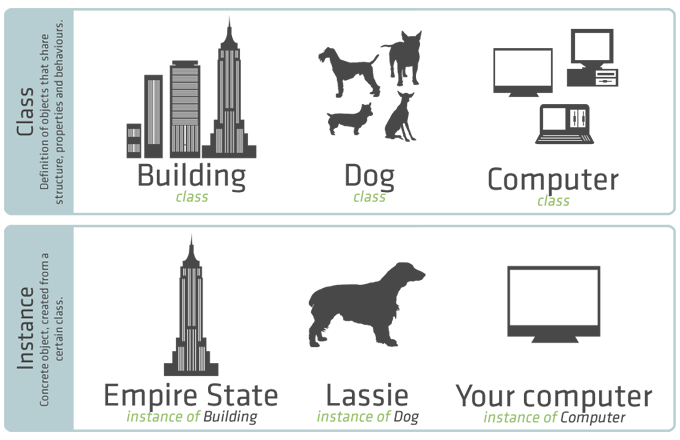
\includegraphics[width=0.8\linewidth]{figures/classes_instances.png}
  \caption{Graphical representation of a class instance.}
  \label{fig:classes}
\end{figure}

To see how they can be defined let's try to code a class representing a person:
\begin{tcolorbox}[breakable, size=fbox, boxrule=1pt, pad at break*=1mm,colback=cellbackground, colframe=cellborder]
\begin{Verbatim}[commandchars=\\\{\}]
\PY{k+kn}{from} \PY{n+nn}{datetime} \PY{k}{import} \PY{n}{date}        

\PY{k}{class} \PY{n+nc}{Person}\PY{p}{:}
\end{Verbatim}
\end{tcolorbox}

First of all, if needed, we have to import the necessary modules, in this case the \texttt{datetime} module is used to managed the person age.
Then the \texttt{class} keyword followed by the class name is used to start the actual class definition.

\subsubsection{The Constructor Method}\label{the-constructor-method}

After declaring the class name, the constructor method must be defined.
In \(\tt{python}\), this is denoted by \texttt{\_\_init\_\_()}
regardless the class name. The \texttt{\_\_init\_\_} function, as every
other method, takes \texttt{self} as the first argument, and then any
number of arguments as desired by the programmer. The \emph{constructor}
allows to specify the initial state of a class by setting its attribute
values. For this example that describes a Person, the programmer wants
to know the name, the birthday and a job (this last one won't be initialize by the constructor).

The \texttt{self} parameter is used to create class attributes. Variables
whose name starts with \texttt{self} have \emph{class scope}, which means are
available within each class method. To use the parameters and
associate them with a particular instance of the class, within the
\texttt{\_\_init\_\_} method, create variables for each argument like
this: \texttt{self.variableName\ =\ param}.

\begin{tcolorbox}[breakable, size=fbox, boxrule=1pt, pad at break*=1mm,colback=cellbackground, colframe=cellborder]
\begin{Verbatim}[commandchars=\\\{\}]
\PY{k+kn}{from} \PY{n+nn}{datetime} \PY{k}{import} \PY{n}{date}

\PY{c+c1}{\PYZsh{} this is the class definition}
\PY{c+c1}{\PYZsh{} usually classes use camel naming convention}
\PY{k}{class} \PY{n+nc}{Person}\PY{p}{:}
    \PY{c+c1}{\PYZsh{} the special method \PYZus{}\PYZus{}init\PYZus{}\PYZus{} allows to instantiate a class}
    \PY{c+c1}{\PYZsh{} with an initial dataset }
    \PY{k}{def} \PY{n+nf}{\PYZus{}\PYZus{}init\PYZus{}\PYZus{}}\PY{p}{(}\PY{n+nb+bp}{self}\PY{p}{,} \PY{n}{name}\PY{p}{,} \PY{n}{birthday}\PY{p}{)}\PY{p}{:}
        \PY{n+nb+bp}{self}\PY{o}{.}\PY{n}{name} \PY{o}{=} \PY{n}{name}
        \PY{n+nb+bp}{self}\PY{o}{.}\PY{n}{birthday} \PY{o}{=} \PY{n}{birthday}     
        \PY{n+nb+bp}{self}\PY{o}{.}\PY{n}{occupation} \PY{o}{=} \PY{k+kc}{None} \PY{c+c1}{\PYZsh{} this attribute not set at instantiation}
\end{Verbatim}
\end{tcolorbox}

Now we that have a class definition that represent a generic person we can 
specialized it to some real person.

\begin{tcolorbox}[breakable, size=fbox, boxrule=1pt, pad at break*=1mm,colback=cellbackground, colframe=cellborder]
\begin{Verbatim}[commandchars=\\\{\}]
\PY{n}{me} \PY{o}{=} \PY{n}{Person}\PY{p}{(}\PY{l+s+s2}{\PYZdq{}}\PY{l+s+s2}{Matteo}\PY{l+s+s2}{\PYZdq{}}\PY{p}{,} \PY{n}{date}\PY{p}{(}\PY{l+m+mi}{1974}\PY{p}{,} \PY{l+m+mi}{10}\PY{p}{,} \PY{l+m+mi}{20}\PY{p}{)}\PY{p}{)}
\PY{n+nb}{print} \PY{p}{(}\PY{n+nb}{type}\PY{p}{(}\PY{n}{me}\PY{p}{)}\PY{p}{)}

<class '\_\_main\_\_.Person'>
\end{Verbatim}
\end{tcolorbox}

Essentially when we instantiate a class \texttt{python} first calls the
\texttt{\_\_init\_\_} method and initializes the class attributes with
the parameter we are passing.

\subsubsection{Class Methods}

We haven't yet defined any "person behaviour", so let's add a couple
of methods to our class, one computing the person's age and the other
setting its primary occupation.

\begin{tcolorbox}[breakable, size=fbox, boxrule=1pt, pad at break*=1mm,colback=cellbackground, colframe=cellborder]
\begin{Verbatim}[commandchars=\\\{\}]
\PY{k}{class} \PY{n+nc}{Person}\PY{p}{:}
    \PY{k}{def} \PY{n+nf}{\PYZus{}\PYZus{}init\PYZus{}\PYZus{}}\PY{p}{(}\PY{n+nb+bp}{self}\PY{p}{,} \PY{n}{name}\PY{p}{,} \PY{n}{birthday}\PY{p}{)}\PY{p}{:}
        \PY{n+nb+bp}{self}\PY{o}{.}\PY{n}{name} \PY{o}{=} \PY{n}{name}
        \PY{n+nb+bp}{self}\PY{o}{.}\PY{n}{birthday} \PY{o}{=} \PY{n}{birthday}     
        \PY{n+nb+bp}{self}\PY{o}{.}\PY{n}{employment} \PY{o}{=} \PY{k+kc}{None}
                
    \PY{c+c1}{\PYZsh{} this is a normal method and will work on some class attribute}
    \PY{k}{def} \PY{n+nf}{age}\PY{p}{(}\PY{n+nb+bp}{self}\PY{p}{,} \PY{n}{d}\PY{o}{=}\PY{n}{date}\PY{o}{.}\PY{n}{today}\PY{p}{(}\PY{p}{)}\PY{p}{)}\PY{p}{:}
        \PY{n}{age} \PY{o}{=} \PY{p}{(}\PY{n}{d} \PY{o}{\PYZhy{}} \PY{n+nb+bp}{self}\PY{o}{.}\PY{n}{birthday}\PY{p}{)}\PY{o}{.}\PY{n}{days}\PY{o}{/}\PY{l+m+mi}{365}
        \PY{n+nb}{print} \PY{p}{(}\PY{l+s+s2}{\PYZdq{}}\PY{l+s+si}{\PYZob{}\PYZcb{}}\PY{l+s+s2}{ is }\PY{l+s+si}{\PYZob{}:.0f\PYZcb{}}\PY{l+s+s2}{ years old}\PY{l+s+s2}{\PYZdq{}}\PY{o}{.}\PY{n}{format}\PY{p}{(}\PY{n+nb+bp}{self}\PY{o}{.}\PY{n}{name}\PY{p}{,} \PY{n}{age}\PY{p}{)}\PY{p}{)}
        
    \PY{k}{def} \PY{n+nf}{mainOccupation}\PY{p}{(}\PY{n+nb+bp}{self}\PY{p}{,} \PY{n}{occupation}\PY{p}{)}\PY{p}{:}
        \PY{n+nb+bp}{self}\PY{o}{.}\PY{n}{employment} \PY{o}{=} \PY{n}{occupation}
        \PY{n+nb}{print} \PY{p}{(}\PY{l+s+s2}{\PYZdq{}}\PY{l+s+si}{\PYZob{}\PYZcb{}}\PY{l+s+s2}{\PYZsq{}}\PY{l+s+s2}{s main occupation is: }\PY{l+s+si}{\PYZob{}\PYZcb{}}\PY{l+s+s2}{\PYZdq{}}\PY{o}{.}\PY{n}{format}\PY{p}{(}\PY{n+nb+bp}{self}\PY{o}{.}\PY{n}{name}\PY{p}{,} \PY{n+nb+bp}{self}\PY{o}{.}\PY{n}{employment}\PY{p}{)}\PY{p}{)}
\end{Verbatim}
\end{tcolorbox}

To access class attributes and methods the $.$ (dot) operator has to be used.

\begin{tcolorbox}[breakable, size=fbox, boxrule=1pt, pad at break*=1mm,colback=cellbackground, colframe=cellborder]
\begin{Verbatim}[commandchars=\\\{\}]
\PY{n}{me}\PY{o}{.}\PY{n}{name}

'Matteo'
\end{Verbatim}
\end{tcolorbox}
        
\begin{tcolorbox}[breakable, size=fbox, boxrule=1pt, pad at break*=1mm,colback=cellbackground, colframe=cellborder]
\begin{Verbatim}[commandchars=\\\{\}]
\PY{n}{me}\PY{o}{.}\PY{n}{age}\PY{p}{(}\PY{n}{date}\PY{o}{.}\PY{n}{today}\PY{p}{(}\PY{p}{)}\PY{p}{)}

Matteo is 46 years old
\end{Verbatim}
\end{tcolorbox}

\subsection{Inheritance and Overriding Methods}\label{inheritance-and-overriding-methods}

Inheritance is basically the idea that different classes can have
similar components, and in order to avoid repeating code, inheritance is
used to link parent classes to descendant classes.

For example, in a fantasy story, there are heroes and monsters but both the heroes and the monsters are characters. And both dragons and orcs are monsters. Though dragons and orcs are different monsters, they share some qualities: they
both have a color, they both have a size, they both have enemies. Orcs
might have characteristics that dragons do not; for example, what kind
of weapon does the orc carry? (Fig.~\ref{fig:inheritance}). Inheritance allows the classes to share information relevant to multiple parts of the code.

\begin{figure}[h]
  \centering
  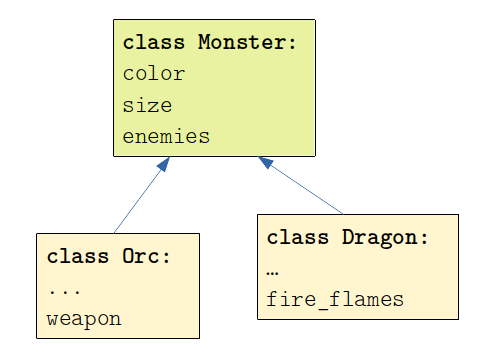
\includegraphics[width=0.5\textwidth]{figures/inheritance.png}
  \caption{Example of inheritance: both \texttt{Dragon} and \texttt{Orc} inherits from \texttt{Monster}, but both add additional attributes that qualify better each "monster features".}
  \label{fig:inheritance}
\end{figure}

Inheritance allows code to be reused and reduces the complexity of a
program. The derived classes (descendants) override or extend the
functionality of base classes (ancestors).
To see how it works in more detail two derived class will be implemented from \texttt{Person}: \texttt{Adult} and \texttt{Child}.

\begin{tcolorbox}[breakable, size=fbox, boxrule=1pt, pad at break*=1mm,colback=cellbackground, colframe=cellborder]
\begin{Verbatim}[commandchars=\\\{\}]

  \PY{k}{class} \PY{n+nc}{Adult}\PY{p}{(}\PY{n}{Person}\PY{p}{)}\PY{p}{:}
    \PY{k}{def} \PY{n+nf}{\PYZus{}\PYZus{}init\PYZus{}\PYZus{}}\PY{p}{(}\PY{n+nb+bp}{self}\PY{p}{,} \PY{n}{name}\PY{p}{,} \PY{n}{birthday}\PY{p}{,} \PY{n}{drv\PYZus{}license\PYZus{}id}\PY{p}{)}\PY{p}{:}
        \PY{n}{Person}\PY{o}{.}\PY{n+nf+fm}{\PYZus{}\PYZus{}init\PYZus{}\PYZus{}}\PY{p}{(}\PY{n+nb+bp}{self}\PY{p}{,} \PY{n}{name}\PY{p}{,} \PY{n}{birthday}\PY{p}{)} \PY{c+c1}{\PYZsh{} this is a special syntax}
        \PY{n+nb+bp}{self}\PY{o}{.}\PY{n}{drv\PYZus{}license\PYZus{}id} \PY{o}{=} \PY{n}{drv\PYZus{}license\PYZus{}id}

        
\PY{k}{class} \PY{n+nc}{Child}\PY{p}{(}\PY{n}{Person}\PY{p}{)}\PY{p}{:}
    \PY{k}{def} \PY{n+nf}{mainOccupation}\PY{p}{(}\PY{n+nb+bp}{self}\PY{p}{)}\PY{p}{:}
        \PY{n+nb+bp}{self}\PY{o}{.}\PY{n}{employment} \PY{o}{=} \PY{l+s+s2}{\PYZdq{}}\PY{l+s+s2}{schoolchild}\PY{l+s+s2}{\PYZdq{}}
        \PY{n+nb}{print} \PY{p}{(}\PY{l+s+s2}{\PYZdq{}}\PY{l+s+si}{\PYZob{}\PYZcb{}}\PY{l+s+s2}{ is a }\PY{l+s+si}{\PYZob{}\PYZcb{}}\PY{l+s+s2}{\PYZdq{}}\PY{o}{.}\PY{n}{format}\PY{p}{(}\PY{n+nb+bp}{self}\PY{o}{.}\PY{n}{name}\PY{p}{,} \PY{n+nb+bp}{self}\PY{o}{.}\PY{n}{employment}\PY{p}{)}\PY{p}{)}
\end{Verbatim}
\end{tcolorbox}

Inheritance is specified in parenthesis after the class name.
\texttt{Child} still inherits from \texttt{Person} and modifies it by setting the only occupation allowed for a child, overriding the \texttt{mainOccupation} method.
\texttt{Adult} class inherits from \texttt{Person} and extends it adding
a new attribute (driving license id). 

\begin{tcolorbox}[breakable, size=fbox, boxrule=1pt, pad at break*=1mm,colback=cellbackground, colframe=cellborder]
\begin{Verbatim}[commandchars=\\\{\}]
\PY{n}{pippo} \PY{o}{=} \PY{n}{Adult}\PY{p}{(}\PY{l+s+s2}{\PYZdq{}}\PY{l+s+s2}{Goofy}\PY{l+s+s2}{\PYZdq{}}\PY{p}{,} \PY{n}{date}\PY{p}{(}\PY{l+m+mi}{1936}\PY{p}{,} \PY{l+m+mi}{1}\PY{p}{,} \PY{l+m+mi}{1}\PY{p}{)}\PY{p}{,} \PY{l+s+s2}{\PYZdq{}}\PY{l+s+s2}{A1234}\PY{l+s+s2}{\PYZdq{}}\PY{p}{)}

\PY{n}{qui} \PY{o}{=} \PY{n}{Child}\PY{p}{(}\PY{l+s+s2}{\PYZdq{}}\PY{l+s+s2}{Huey}\PY{l+s+s2}{\PYZdq{}}\PY{p}{,} \PY{n}{date}\PY{p}{(}\PY{l+m+mi}{2014}\PY{p}{,} \PY{l+m+mi}{10}\PY{p}{,} \PY{l+m+mi}{9}\PY{p}{)}\PY{p}{)}
\end{Verbatim}
\end{tcolorbox}

Behind the scenes, when instantiating a \texttt{Child} class, the constructor of \texttt{Person} is called and the attributes, \texttt{name} and \texttt{birthday} are initialised.  

For the \texttt{Adult} class things are a little bit different because a new attribute has been added, so we need to code its own constructor where we first call explicitly the \texttt{Person}'s constructor (\texttt{Person.\_\_init\_\_(self,$\ldots$)} and then we initialise the new attribute.

\begin{tcolorbox}[breakable, size=fbox, boxrule=1pt, pad at break*=1mm,colback=cellbackground, colframe=cellborder]
\begin{Verbatim}[commandchars=\\\{\}]
\PY{n}{pippo}\PY{o}{.}\PY{n}{age}\PY{p}{(}\PY{p}{)}
\PY{n}{pippo}\PY{o}{.}\PY{n}{mainOccupation}\PY{p}{(}\PY{l+s+s2}{\PYZdq{}}\PY{l+s+s2}{Comic}\PY{l+s+s2}{\PYZsq{}}\PY{l+s+s2}{s character}\PY{l+s+s2}{\PYZdq{}}\PY{p}{)}

Goofy is 85 years old
Goofy's main occupation is: Comic's character
\end{Verbatim}
\end{tcolorbox}

\begin{tcolorbox}[breakable, size=fbox, boxrule=1pt, pad at break*=1mm,colback=cellbackground, colframe=cellborder]
\begin{Verbatim}[commandchars=\\\{\}]
\PY{n}{qui}\PY{o}{.}\PY{n}{age}\PY{p}{(}\PY{p}{)}
\PY{n}{qui}\PY{o}{.}\PY{n}{mainOccupation}\PY{p}{(}\PY{p}{)}

Huey is 6 years old
Huey is a schoolchild
\end{Verbatim}
\end{tcolorbox}
